%% ****** Start of file apstemplate.tex ****** %
%%
%%
%%   This file is part of the APS files in the REVTeX 4 distribution.
%%   Version 4.1r of REVTeX, August 2010
%%
%%
%%   Copyright (c) 2001, 2009, 2010 The American Physical Society.
%%
%%   See the REVTeX 4 README file for restrictions and more information.
%%
%
% This is a template for producing manuscripts for use with REVTEX 4.0
% Copy this file to another name and then work on that file.
% That way, you always have this original template file to use.
%
% Group addresses by affiliation; use superscriptaddress for long
% author lists, or if there are many overlapping affiliations.
% For Phys. Rev. appearance, change preprint to twocolumn.
% Choose pra, prb, prc, prd, pre, prl, prstab, prstper, or rmp for journal
%  Add 'draft' option to mark overfull boxes with black boxes
%  Add 'showpacs' option to make PACS codes appear
%  Add 'showkeys' option to make keywords appear
\documentclass[aps,pre,preprint,groupedaddress]{revtex4-1}
%\documentclass[aps,prl,preprint,superscriptaddress]{revtex4-1}
%\documentclass[aps,prl,reprint,groupedaddress]{revtex4-1}

% You should use BibTeX and apsrev.bst for references
% Choosing a journal automatically selects the correct APS
% BibTeX style file (bst file), so only uncomment the line
% below if necessary.
\bibliographystyle{apsrev4-1}
\usepackage{graphicx}
\usepackage{float}
\usepackage{amsmath}

\begin{document}

% Use the \preprint command to place your local institutional report
% number in the upper righthand corner of the title page in preprint mode.
% Multiple \preprint commands are allowed.
% Use the 'preprintnumbers' class option to override journal defaults
% to display numbers if necessary
%\preprint{}

%Title of paper
\title{\textbf{Topological Mechanics and Topological Phononic Phases}}

% repeat the \author .. \affiliation  etc. as needed
% \email, \thanks, \homepage, \altaffiliation all apply to the current
% author. Explanatory text should go in the []'s, actual e-mail
% address or url should go in the {}'s for \email and \homepage.
% Please use the appropriate macro foreach each type of information

% \affiliation command applies to all authors since the last
% \affiliation command. The \affiliation command should follow the
% other information
% \affiliation can be followed by \email, \homepage, \thanks as well.
\author{Shang Zhang}
%\email[]{Your e-mail address}
%\homepage[]{Your web page}
%\thanks{}
%\altaffiliation{}
\affiliation{Department of Physics, University of Michigan}

%Collaboration name if desired (requires use of superscriptaddress
%option in \documentclass). \noaffiliation is required (may also be
%used with the \author command).
%\collaboration can be followed by \email, \homepage, \thanks as well.
%\collaboration{}
%\noaffiliation

\date{\today}

\begin{abstract}
Electronic topological insulators have inspired the design of new mechanical systems that could soon find real-life applications.
\end{abstract}

% insert suggested PACS numbers in braces on next line
\pacs{}
% insert suggested keywords - APS authors don't need to do this
%\keywords{}

%\maketitle must follow title, authors, abstract, \pacs, and \keywords
\maketitle

% body of paper here - Use proper section commands
% References should be done using the \cite, \ref, and \label commands
\section{Introduction}
% Put \label in argument of \section for cross-referencing
%\section{\label{}}
Creating artificial materials that control electrons, photons, sound waves or mechanical energy is a prime focus of modern materials science. In the past few years, a new paradigm is emerging with the application of ideas from topology, the mathematics describing properties that are unchanged by smooth deformations. People discovered interesting phenomenology of electrons in topological insulators, which are a kind of material with non-trivial topological order that behaves as an insulator in its interior but whose surface contains conducting states, meaning that electrons can only move along the surface of the material\cite{cite-key1,cite-key2,cite-key3}.

Following an explosion of studying in topological phases in hard condensed matter, this topological approach has recently been used from the quantum realm of electrons to the world of classical mechanical systems.  Electronic topological insulators have inspired the design of new topological mechanical systems that could lead to new design principles for metamaterials\cite{huber2016topological}. In this review, we will try to establish the connections between topological electrons systems to classical mechanical systems based on recent research work, as well as perspectives in this field.

\subsection{Analogy between Quantum and Newton's Mechanics}

At first sight, electronic systems described by quantum mechanics seem totally different to mechanical modes or phonons described by Newton's equations of motion. But it is not always the case.

In 1985, it was discovered that similar geometric phases to Berry's phase \cite{cite-key5} occurred in classical systems with single or few mechanical modes \cite{cite-key9}, which illustrates the appearing of geometric nature of phases in classical systems.

Then with the emergence of topological insulator, it turned out that the bulk and edge states of phononic systems can display the same unusual properties seen in the topological insulators\cite{cite-key11,cite-key12}. So it seems clearer to us that there's some analogy between quantum and newton's mechanics that introduces the similar topological properties in electronic and phononic systems.

To illustrate the analogy between quantum and Newton's mechanics, consider the equation of motions in a set of coupled simple harmonic oscillators,
\begin{align}
\ddot{x}_i &= -D_{ij}x_j+A_{ij}\dot{x}_j
\label{eq1}
\end{align}

Where the dynamical matrix $D$ is real and positive definite, and the skew-symmetric $A$ describes the coupling between velocities and positions. Then one can rewrite equation (\ref{eq1}) to,

\begin{align}
i\frac{\partial}{\partial t}
\begin{pmatrix}
\sqrt{D}^{T}x\\
i\dot{x}
\end{pmatrix}
&=
\begin{pmatrix}
0 & \sqrt{D}^{T}\\
\sqrt{D} & iA
\end{pmatrix}
\begin{pmatrix}
\sqrt{D}^{T}x\\
i\dot{x}
\end{pmatrix}
\label{eq2}
\end{align}

Equation (\ref{eq2}) transfers Newton's equations into Hermitian eigenvalue equations, in similar form to Schrodinger equation.

\begin{figure}
\centering
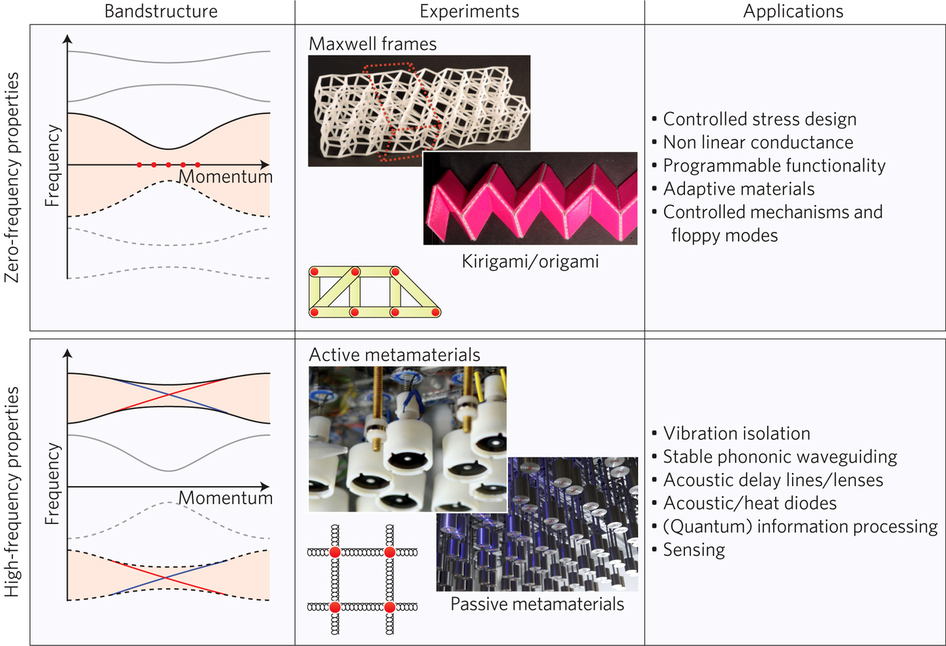
\includegraphics[scale=0.4]{nphys3801-f1.jpg}
\caption{\label{}}
\end{figure}

Three routes to present topological mechanical systems,
\begin{itemize}
\item Capitalize on the intrinsic particle–hole symmetry
\item Engineer a topological dynamical matrix $D$ directly
\item A properly engineered $A$ can give rise to systems with broken time-reversal symmetry, described by a Chern number
\end{itemize}

\section{Zero-frequency}

\section{High-frequency}

% If in two-column mode, this environment will change to single-column
% format so that long equations can be displayed. Use
% sparingly.
%\begin{widetext}
% put long equation here
%\end{widetext}

% figures should be put into the text as floats.
% Use the graphics or graphicx packages (distributed with LaTeX2e)
% and the \includegraphics macro defined in those packages.
% See the LaTeX Graphics Companion by Michel Goosens, Sebastian Rahtz,
% and Frank Mittelbach for instance.
%
% Here is an example of the general form of a figure:
% Fill in the caption in the braces of the \caption{} command. Put the label
% that you will use with \ref{} command in the braces of the \label{} command.
% Use the figure* environment if the figure should span across the
% entire page. There is no need to do explicit centering.

% Surround figure environment with turnpage environment for landscape
% figure
% \begin{turnpage}
% \begin{figure}
% \includegraphics{}%
% \caption{\label{}}
% \end{figure}
% \end{turnpage}

% tables should appear as floats within the text
%
% Here is an example of the general form of a table:
% Fill in the caption in the braces of the \caption{} command. Put the label
% that you will use with \ref{} command in the braces of the \label{} command.
% Insert the column specifiers (l, r, c, d, etc.) in the empty braces of the
% \begin{tabular}{} command.
% The ruledtabular enviroment adds doubled rules to table and sets a
% reasonable default table settings.
% Use the table* environment to get a full-width table in two-column
% Add \usepackage{longtable} and the longtable (or longtable*}
% environment for nicely formatted long tables. Or use the the [H]
% placement option to break a long table (with less control than 
% in longtable).
% \begin{table}%[H] add [H] placement to break table across pages
% \caption{\label{}}
% \begin{ruledtabular}
% \begin{tabular}{}
% Lines of table here ending with \\
% \end{tabular}
% \end{ruledtabular}
% \end{table}

% Surround table environment with turnpage environment for landscape
% table
% \begin{turnpage}
% \begin{table}
% \caption{\label{}}
% \begin{ruledtabular}
% \begin{tabular}{}
% \end{tabular}
% \end{ruledtabular}
% \end{table}
% \end{turnpage}

% Specify following sections are appendices. Use \appendix* if there
% only one appendix.
%\appendix
%\section{}

% If you have acknowledgments, this puts in the proper section head.
%\begin{acknowledgments}
% put your acknowledgments here.
%\end{acknowledgments}

% Create the reference section using BibTeX:
\bibliography{TermPaper}

\end{document}
%
% ****** End of file apstemplate.tex ******

